\part{Methodology}
In this part we will discuss all the procedure that took place from building our testing platform, based on the Rover Mini and the sensors used. Setting up the Nav2 navigation stack. The procedure used to port the Global planner from ROS 1 to ROS 2. How we integrate the system and the software that is used to setup the Open-RMF system.
\chapter{Description of research platform and hardware used}
The robot is a 4 wheel drive (WD) skid-steering (see Figure \ref{fig:RoverRobotics Rover Mini})that has a maximum speed of 12.87 km/h with a payload of 45,36 kg. With an operating time of Operating Time 60-90 minutes active or max 6 hours in idle. The company offer the code to control it and also to simulate on Gazebo on github\footnote{\href{https://github.com/RoverRobotics/roverrobotics_ros2}{https://github.com/RoverRobotics/roverrobotics\_ros2}}. The code is steel tested only for ROS 2 Humble, this is going to be our version of ROS 2 that we are going to use for navigation on the Rover.\\
For controlling it, the rover give a USB terminal for connecting to a PC or single board computer. For this purpose we are using a Mini PC where there is all the control of all the navigation based on Nav2.
The Mini PC is a Beelink SER3-E-16512EJ0W64PRO with a Ryzen 7 3750H Picasso processor which is a quad-core 8-thread 2.3 GHz mobile processor boosting to 4.0 GHz with Radeon RX Vega 10 Graphics.
The power that it's necessary from it to work will be took from the Rover that can provide 19V.
\begin{figure}[h]
	\centering
	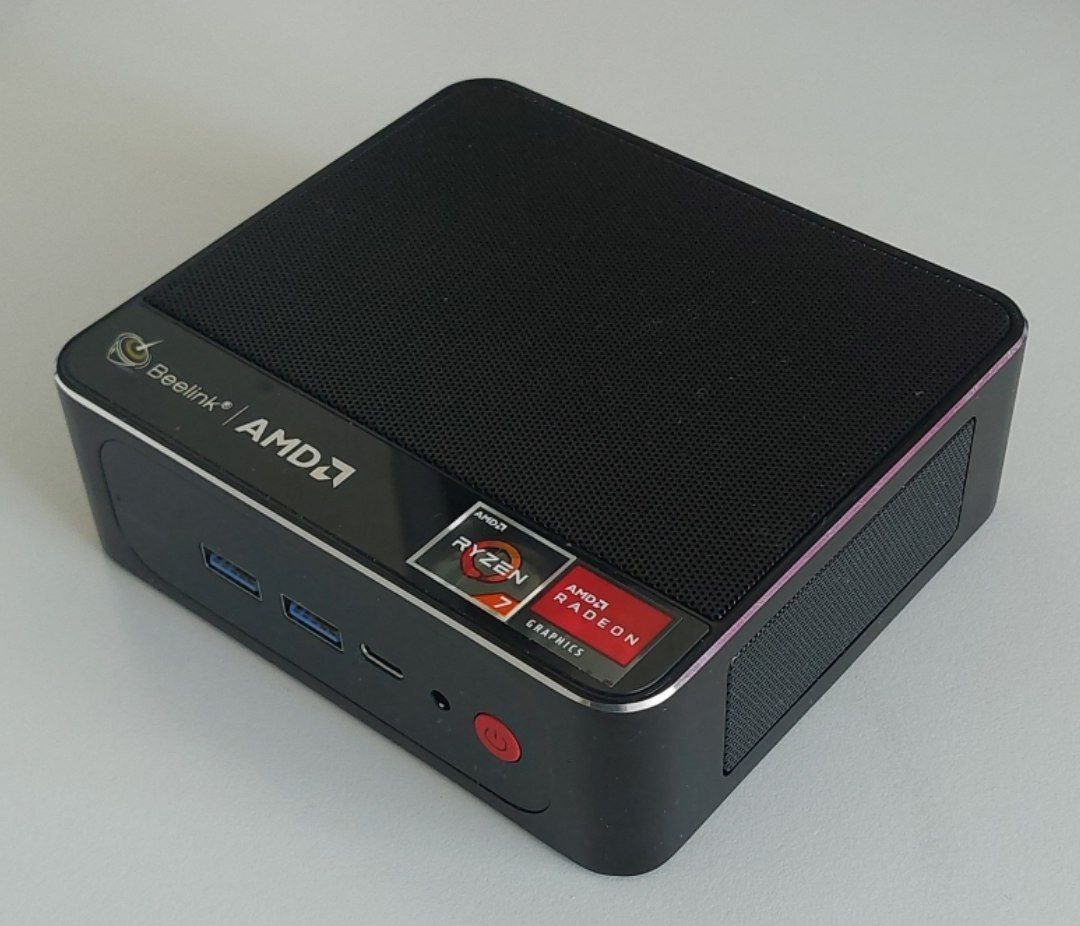
\includegraphics[width=0.4\linewidth]{img/miniPC.jpg}
	\captionof{figure}{Mini PC used}
\end{figure}\\
On top of that to increase the estimation of odometry we will mount an IMU Witmotion (WIT) JY901B. A 9-Axis Combined IMU/Magnetometer/Altimeter (linear accelerations, angular velocities, Euler angles, magnetic field, barometry, altitude). The data from the sensor use a TTL/UART protocol that are collected using the libeary Witmotion Sensors UART Connection Library\cite{andrei_vukolov_2022_7017118},using a channel bridge chip USB to serial, and then published into ROS 2 ecosystem through a node \texttt{witmotion\_ros} using the code from this repo in github ElettraSciComp/witmotion\_IMU\_ros\footnote{\href{https://github.com/ElettraSciComp/witmotion_IMU_ros/tree/ros2}{https://github.com/ElettraSciComp/witmotion\_IMU\_ros/tree/ros2}}.
\begin{figure}[h]
	\centering
	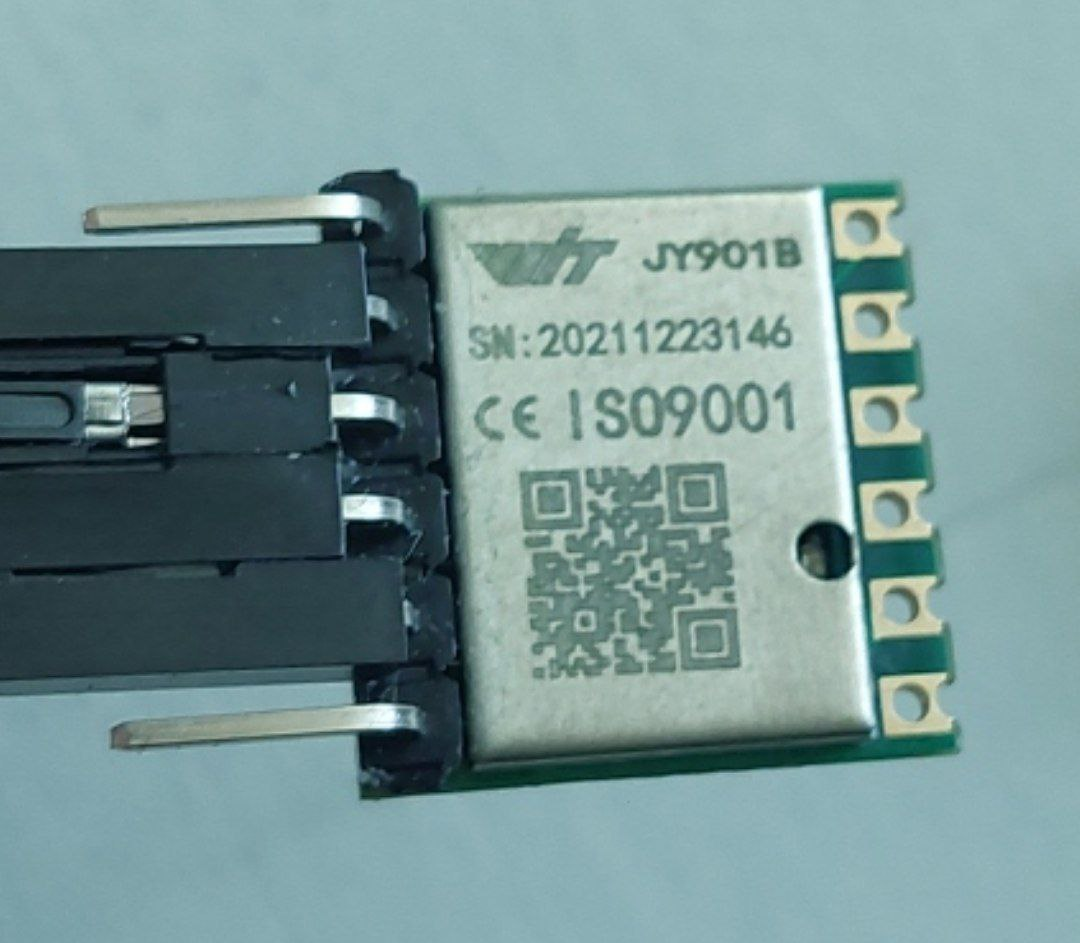
\includegraphics[width=0.4\linewidth]{img/IMU.jpg}
	\captionof{figure}{IMU used}
\end{figure}\\
The last sensor necessary to complete the navigation that is used in localization as described in \ref{ref_map_to_odom} to generate a link between the TF frame \texttt{map} and \texttt{odom} that compensate the errors generated by the model before and see obstacles is a Laser 2D scan because gives as information in all the directions using only a sensor and we built have built only a 2D map, respect at other tools are available \cite{10056144}\cite{vslamComparison2021} that may require more computer power.
The Laser scan used is RPLIDAR S1, 360 degree 2D laser scanner
(LIDAR that is light detection and ranging) with a distance range of 40m on white object and 10m on black ones, a sample rate of 9.2kHz, scan rate from 8 to 15 Hz, so an angular resolution of 0.313-0.587°, accuracy of $\pm$5cm and resolution of 3cm.
The code is available on github Slamtec/sllidar\_ros2 \footnote{\href{https://github.com/Slamtec/sllidar_ros2}{https://github.com/Slamtec/sllidar\_ros2}}.
\begin{figure}[h]
	\centering
	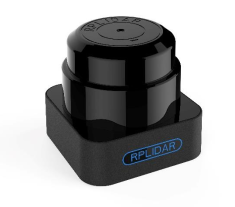
\includegraphics[width=0.4\linewidth]{img/laserScanRPLIDAR.png}
	\captionof{figure}{LIDAR used}
\end{figure}\\
Then all is mounted on the Rover as in the following picture. The couse for this topology is that:
\begin{figure}[h]
	\centering
	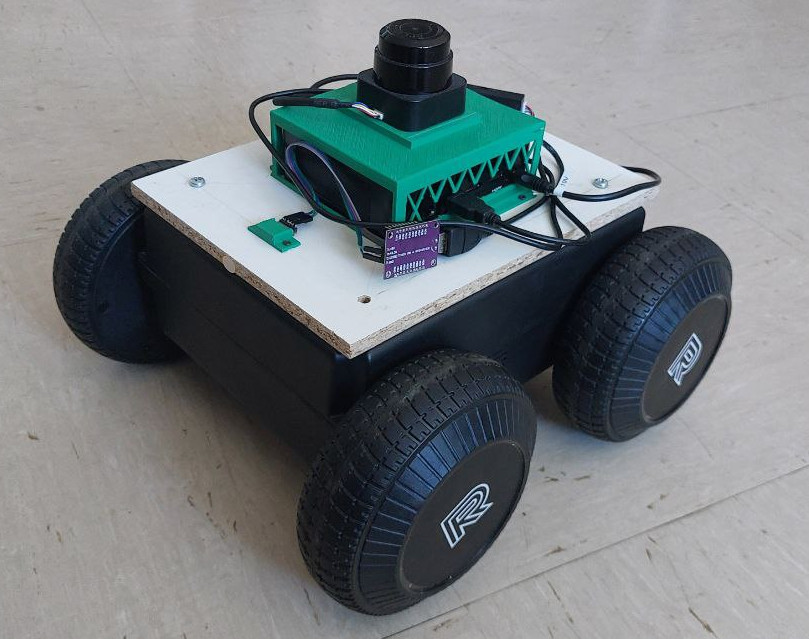
\includegraphics[width=0.4\linewidth]{img/RoverwithSensor.jpg}
	\captionof{figure}{LIDAR used}
\end{figure}\\
\chapter{Steps taken to port the navigation stack from ROS 1 to ROS 2}
\chapter{Hardware adaptation process from Rover Zero to Rover Mini}
\chapter{Integration of the navigation stack with Open-RMF}
\chapter{Testing and evaluation of the system}


